\documentclass{beamer}\usepackage[]{graphicx}\usepackage[]{color}
%% maxwidth is the original width if it is less than linewidth
%% otherwise use linewidth (to make sure the graphics do not exceed the margin)
\makeatletter
\def\maxwidth{ %
  \ifdim\Gin@nat@width>\linewidth
    \linewidth
  \else
    \Gin@nat@width
  \fi
}
\makeatother

\definecolor{fgcolor}{rgb}{0.345, 0.345, 0.345}
\newcommand{\hlnum}[1]{\textcolor[rgb]{0.686,0.059,0.569}{#1}}%
\newcommand{\hlstr}[1]{\textcolor[rgb]{0.192,0.494,0.8}{#1}}%
\newcommand{\hlcom}[1]{\textcolor[rgb]{0.678,0.584,0.686}{\textit{#1}}}%
\newcommand{\hlopt}[1]{\textcolor[rgb]{0,0,0}{#1}}%
\newcommand{\hlstd}[1]{\textcolor[rgb]{0.345,0.345,0.345}{#1}}%
\newcommand{\hlkwa}[1]{\textcolor[rgb]{0.161,0.373,0.58}{\textbf{#1}}}%
\newcommand{\hlkwb}[1]{\textcolor[rgb]{0.69,0.353,0.396}{#1}}%
\newcommand{\hlkwc}[1]{\textcolor[rgb]{0.333,0.667,0.333}{#1}}%
\newcommand{\hlkwd}[1]{\textcolor[rgb]{0.737,0.353,0.396}{\textbf{#1}}}%

\usepackage{framed}
\makeatletter
\newenvironment{kframe}{%
 \def\at@end@of@kframe{}%
 \ifinner\ifhmode%
  \def\at@end@of@kframe{\end{minipage}}%
  \begin{minipage}{\columnwidth}%
 \fi\fi%
 \def\FrameCommand##1{\hskip\@totalleftmargin \hskip-\fboxsep
 \colorbox{shadecolor}{##1}\hskip-\fboxsep
     % There is no \\@totalrightmargin, so:
     \hskip-\linewidth \hskip-\@totalleftmargin \hskip\columnwidth}%
 \MakeFramed {\advance\hsize-\width
   \@totalleftmargin\z@ \linewidth\hsize
   \@setminipage}}%
 {\par\unskip\endMakeFramed%
 \at@end@of@kframe}
\makeatother

\definecolor{shadecolor}{rgb}{.97, .97, .97}
\definecolor{messagecolor}{rgb}{0, 0, 0}
\definecolor{warningcolor}{rgb}{1, 0, 1}
\definecolor{errorcolor}{rgb}{1, 0, 0}
\newenvironment{knitrout}{}{} % an empty environment to be redefined in TeX

\usepackage{alltt}
\usepackage{xcolor}
\usepackage{graphicx}
\usepackage{tikz}
\usetikzlibrary{shapes.geometric, arrows}
\usepackage{verbatim}
\definecolor{UAred}{RGB}{204,0,51}
\definecolor{UAblue}{RGB}{0,51,102}

\useoutertheme{infolines}%makes informative footer
\usetheme{Pittsburgh}
\setbeamercolor{structure}{fg=UAblue}
\setbeamercolor{normal text}{fg=black}
\setbeamercolor{upper separation line head}{bg=UAred}
\AtBeginSection{\frame{\sectionpage}}%make section title pages
\AtBeginSubsection{\frame{\subsectionpage}}

\setbeamertemplate{headline}
{
  \leavevmode
  \hbox{
  \begin{beamercolorbox}[wd=.5\paperwidth,ht=6ex,dp=2ex,left,rightskip=1em]{section in head/foot}%
    \usebeamerfont{subsection in head/foot}\hspace*{2ex}\insertshorttitle
  \end{beamercolorbox}
  \begin{beamercolorbox}[wd=.25\paperwidth,ht=6ex,dp=1ex,left,leftskip=1em]{subsection in head/foot}%
    \usebeamerfont{section in head/foot}\insertsectionhead\hspace*{2ex}
  \end{beamercolorbox}
  \begin{beamercolorbox}[wd=.25\paperwidth,ht=6ex,dp=1ex,right,leftskip=1em]{subsection in head/foot}%
    
\includegraphics[scale=.15]{./Figures/UA_CPH_RGB_Primary.png}
  \end{beamercolorbox}}
  \begin{beamercolorbox}[colsep=1.5pt,ht=.75ex]{upper separation line head}
  \end{beamercolorbox}
  \vskip0pt%
}

\setbeamertemplate{footline}
{
  \leavevmode
  \hbox{%

\begin{beamercolorbox}[wd=.70\paperwidth,ht=4.25ex,dp=4ex,left,leftskip=2ex]{title in head/foot}%
    \usebeamerfont{title in head/foot}\insertshorttitle{} - \insertshortauthor
\end{beamercolorbox}%
\begin{beamercolorbox}[wd=.20\paperwidth,ht=4.25ex,dp=4ex,center]{date in head/foot}%
    \usebeamerfont{date in head/foot}\insertshortdate{}
\end{beamercolorbox}%
\begin{beamercolorbox}[wd=.10\paperwidth,ht=4.25ex,dp=4ex,right,rightskip=2ex]{date in head/foot}%
    \insertframenumber{} / \inserttotalframenumber
  \end{beamercolorbox}}%
\vskip0pt%
}



\setbeamertemplate{frametitle}{%place the title in the center

\vspace*{4mm}\hspace*{-2mm}\insertframetitle

}


\setbeamertemplate{navigation symbols}{}%remove Navigation Symbols
%start entering presentation specific stuff below here...
%start entering presentation specific stuff below here...%%%%%%%%%%%%%%%%%%%%%%%%%%%%%%%%%%%%%%%%%%%%%%%


\title[Interactive Documents and Applications]{Interactive Documents and Applications with R}
\author[Dominic LaRoche]{Dominic LaRoche}
\IfFileExists{upquote.sty}{\usepackage{upquote}}{}
\begin{document}

\maketitle

\begin{frame}{Outline}
\begin{itemize}
\item Introduction
\bigskip
\item Example document and example application 
\bigskip
\item Nuts and Bolts
\end{itemize}
\end{frame}

\section{Introduction}

\begin{frame}{What are interactive documents and applications?}
Interactive documents and applications are graphical user interfaces which run analyses in the background.
\bigskip
\begin{itemize}
\item Allow user to interact with analyses
\bigskip
\item Run pre-defined analyses
\bigskip
\item Provide results
\end{itemize}
\end{frame}

\begin{frame}{How are interactive documents and applications beneficial?}
Interactive Applications:
\begin{itemize}
\smallskip
\item Streamline repetetive analyses and reduce errors
\smallskip
\pause
\item Increase efficiency of an organization by enabling others to perform and interpret simple analyses
\smallskip
\pause
\item Provide a high-value service to customers
\end{itemize}
\bigskip
\pause

Interactive Documents:
\smallskip
\begin{itemize}
\item Provide a tool to both inform \emph{and} educate
\smallskip
\pause
\item Allow users to ask and answer their own questions
  \begin{itemize}
  \item Facilitate discovery
  \item Understand the ``why" and not just the ``what"
  \end{itemize}
\end{itemize}
\end{frame}

\begin{frame}{How are interactive documents and applications beneficial?}
Other potential uses:
\bigskip
\begin{itemize}
\item Teaching
\bigskip
\pause
\item Marketing
\bigskip
\pause
\item Public health
\end{itemize}
\end{frame}


\begin{frame}{Interactive Applications}
Written in R:
\begin{itemize}
\item Can do anything you can do in R
\smallskip
\item Large library of pre-written widgets for user interaction
\smallskip
\item Can accomodate anything you can write in HTML, Java, Python, etc.
\smallskip
\item Can be hosted locally and run behind a firewall
\smallskip
\item Use shiny.io for free (up to 5 apps)
\end{itemize}
\end{frame}

\begin{frame}{Interactive Reports}
Written in Rmarkdown:
\begin{itemize}
\item Combines report text and code into a single document
\smallskip
\item Can do anything you can do in R 
\smallskip
\item Felixble formatting
\smallskip
\item Can easily convert between document types
\smallskip
\item Can create a static document from interactive one
\smallskip
\item Document must be hosted
\pause
  \begin{itemize}
  \item On the web
  \item Locally as application
  \end{itemize}
\end{itemize}
\end{frame}

\section{Examples}

\begin{frame}{Examples}
\begin{itemize}
\item Interactive Application
\bigskip
\item Interactive Document
\bigskip
\item Shiny Example Library
\end{itemize}
\end{frame}

\section{Nuts and Bolts}

\begin{frame}{WARNING!}
I will be discussing some details of creating these type of applications and documents which will involve talking about code and programming.\\ Feel free to escape!
\end{frame}

\begin{frame}{Architecture of an Application}
\begin{center}
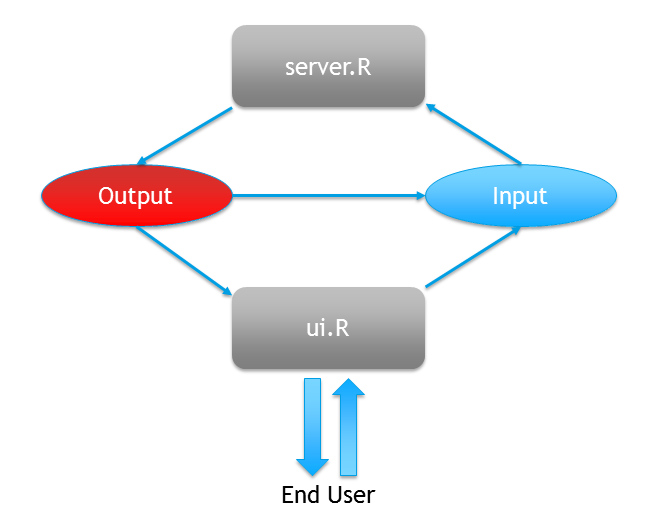
\includegraphics[scale=.4]{./Figures/FullArchitecture}
\end{center}
\end{frame}

\begin{frame}{Building an Application}
Applications depend on two main objects:
\bigskip
\begin{itemize}
\item input
  \begin{itemize}
  \item Stores all the user inputs for use in the analysis
  \item Data, parameters, etc.
  \end{itemize}
\pause
\bigskip
\item output
  \begin{itemize}
  \item Stores all of the outputs from the analysis
  \item Everything returned to the user
  \end{itemize}
\end{itemize}
\end{frame}

\begin{frame}{Building an Application}
Applications use two main functions from the shiny package:
\bigskip
\begin{itemize}
\item ShinyServer
  \begin{itemize}
  \item Controls the server logic
    \begin{itemize}
    \item What happens and in what order
    \end{itemize}
  \item Calls sub-functions or other programs
  \item Creates dynamic inputs
  \item uses ``inputs" to create ``outputs"
  \end{itemize}
\pause
\bigskip
\item ShinyUI
  \begin{itemize}
  \item Defines the appearance of the application
  \item Interacts with the user to collect ``inputs"
  \item Displays all the ``outputs" of the analysis
  \end{itemize}
\end{itemize}
\end{frame}

\begin{frame}{Pre-packaged Inputs}

\end{frame}


\begin{frame}{Pre-pacakged Outputs}

\end{frame}

\begin{frame}{Reactivity}
The analysis must respond to updated user inputs.  This is known as \textbf{reactivity}.
\begin{itemize}
\bigskip
\item 3 main components for reactivity
  \begin{itemize}
  \item[1.)] Reactive source (generally an input)
  \item[2.)] Reactive conductor (usually a function)*
  \item[3.)] Reactive endpoint (usually an output)
  \end{itemize}
  \bigskip
\item Trickiest part for typical R programmer
\bigskip
\item All manipulations of reactive values must be done inside the reactive environment
\end{itemize}
\end{frame}

\begin{frame}{Reactivity}
Some of the tricky things about reactivity:
\begin{itemize}
\item A reactive function will not execute if there is no reactive endpoint
\pause
\bigskip
\item A reactive value is always reacting to user inputs
  \begin{itemize}
  \smallskip
  \item Some inputs may have no initial value
  \smallskip
  \item Other inputs may require typing
  \end{itemize}
\pause
\bigskip
\item Can use observer() function as an endpoint if no output is required
\pause
\bigskip
\item isolate() function + action button can control unwanted reactivity
\bigskip
\pause
\item validate() function can require certain conditions are met before reacting
\end{itemize}
\end{frame}


\begin{frame}{Dynamic Applications}
Extensive applications should be dynamic
\bigskip
\begin{itemize}
\item Limit the number of inputs to focus the user
\pause
\bigskip
\item Ask for inputs as needed and build up options
\pause
\bigskip
\item Make inputs from reactive outputs
\end{itemize}
\end{frame}


\begin{frame}{Building an Interactive Document}
Interactive document is a special case of an application
\pause
\bigskip
\begin{itemize}
\item Written in Rmarkdown
  \begin{itemize}
  \item Markup language (think \LaTeX) that weaves code and text into single document
  \end{itemize}
\pause
\bigskip
\item Output controlled by header: word, pdf, latex presentation, io slides, and HTML
\bigskip
\pause
\item Specify HTML with shiny runtime to get interactive document.
\end{itemize}  
\end{frame}


\begin{frame}{Building an Interactive Document}
Some differences from a standard application:
\bigskip
\pause
\begin{itemize}
\item Only 1 file (no separate server.R and ui.R files)
\pause
\bigskip
\item Use inputPanel instead of shinyUI() function
\bigskip
\pause
\item Outputs are rendered in 2 stages:
  \smallskip
  \begin{itemize}
  \item[1.)] Rendered into HTML by shiny package
  \smallskip
  \item[2.)] Placed into document via Rmarkdown arguments
  \end{itemize}
\end{itemize}
\end{frame}

\begin{frame}{Questions?}
\begin{center}
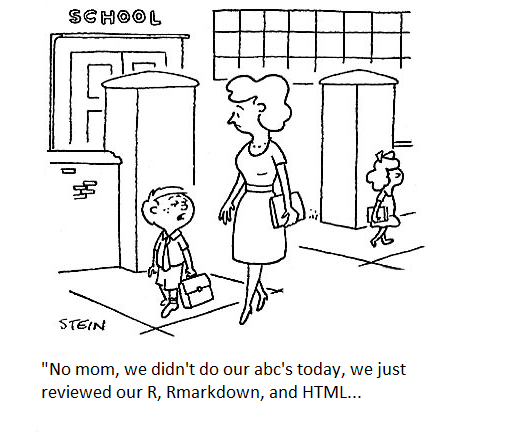
\includegraphics[scale=.5]{./Figures/codingcartoon.png}
\end{center}
\end{frame}
\end{document}
